\chapter{Profiling Benchmark Applications} \label{hdrnn-profile}

Flame graphs capturing application performance during a single epoch are listed below

\subsection*{Flame graphs from perf Measurements}

\begin{figure}[H]
	\centering
	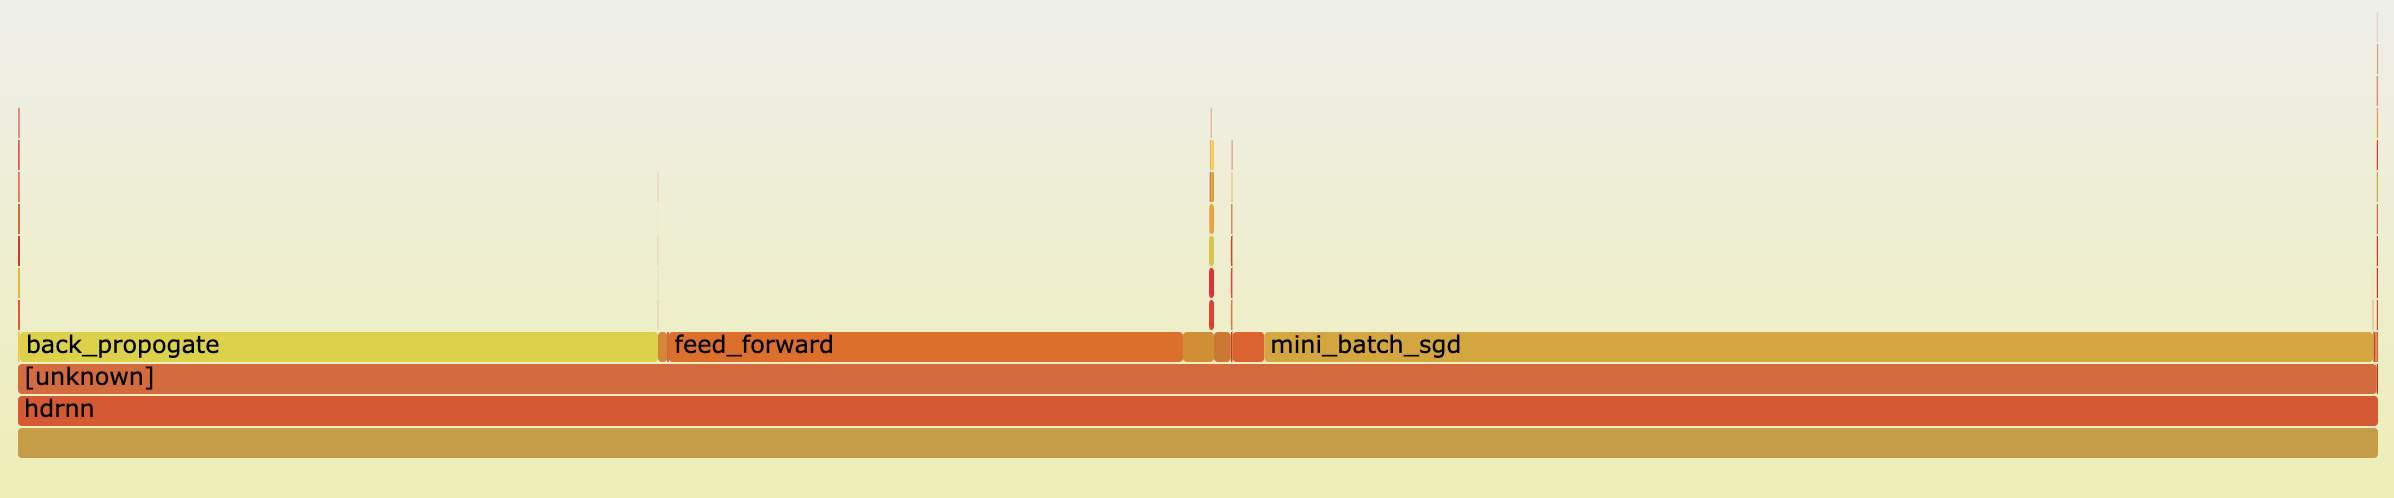
\includegraphics[scale=0.34]{c-math.h-fg.png}
	\caption{c-math.h}
\end{figure}

\begin{figure}[H]
	\centering
	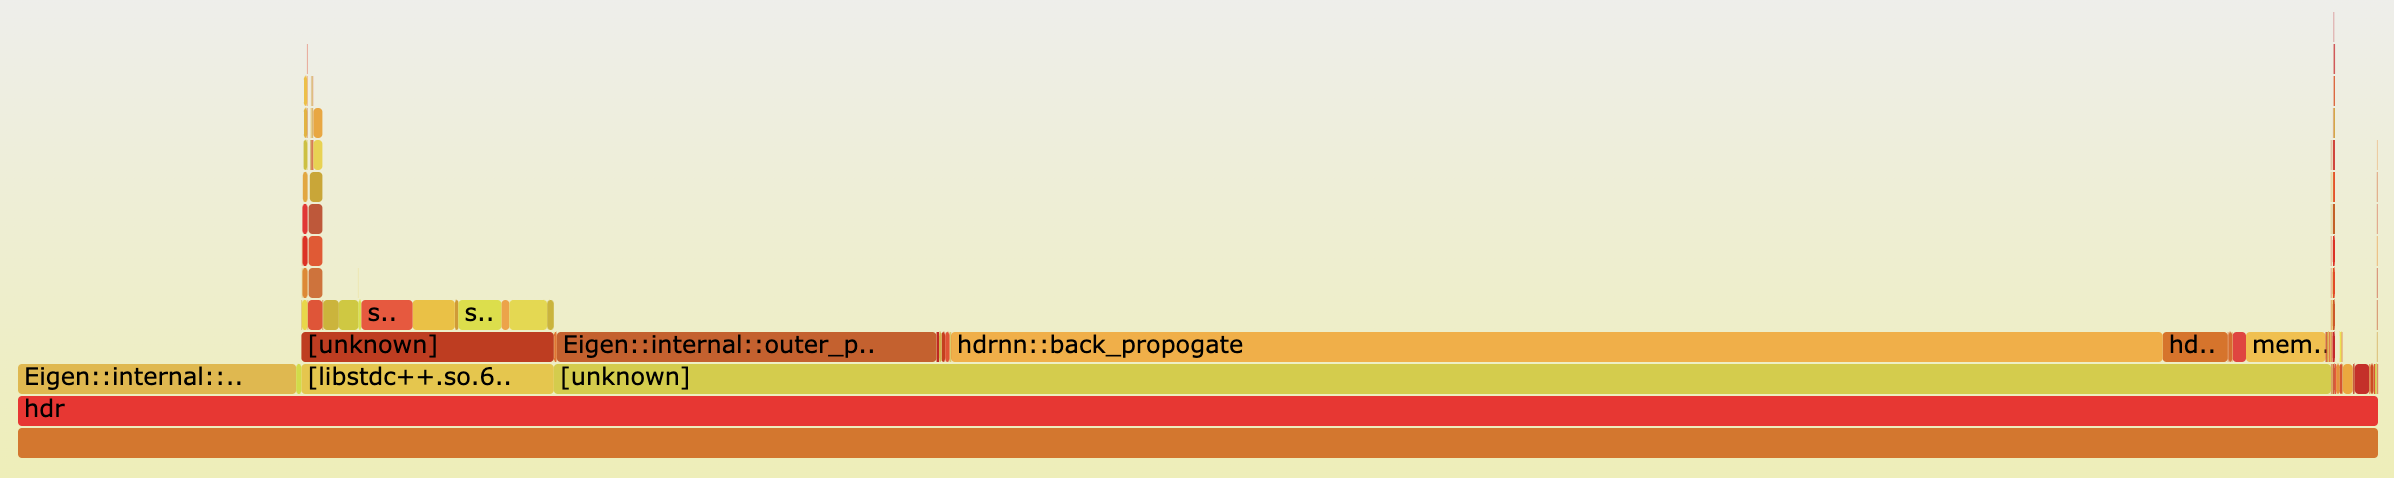
\includegraphics[scale=0.34]{cpp-eigen-fg.png}
	\caption{cpp-eigen}
\end{figure}

\begin{figure}[H]
	\centering
	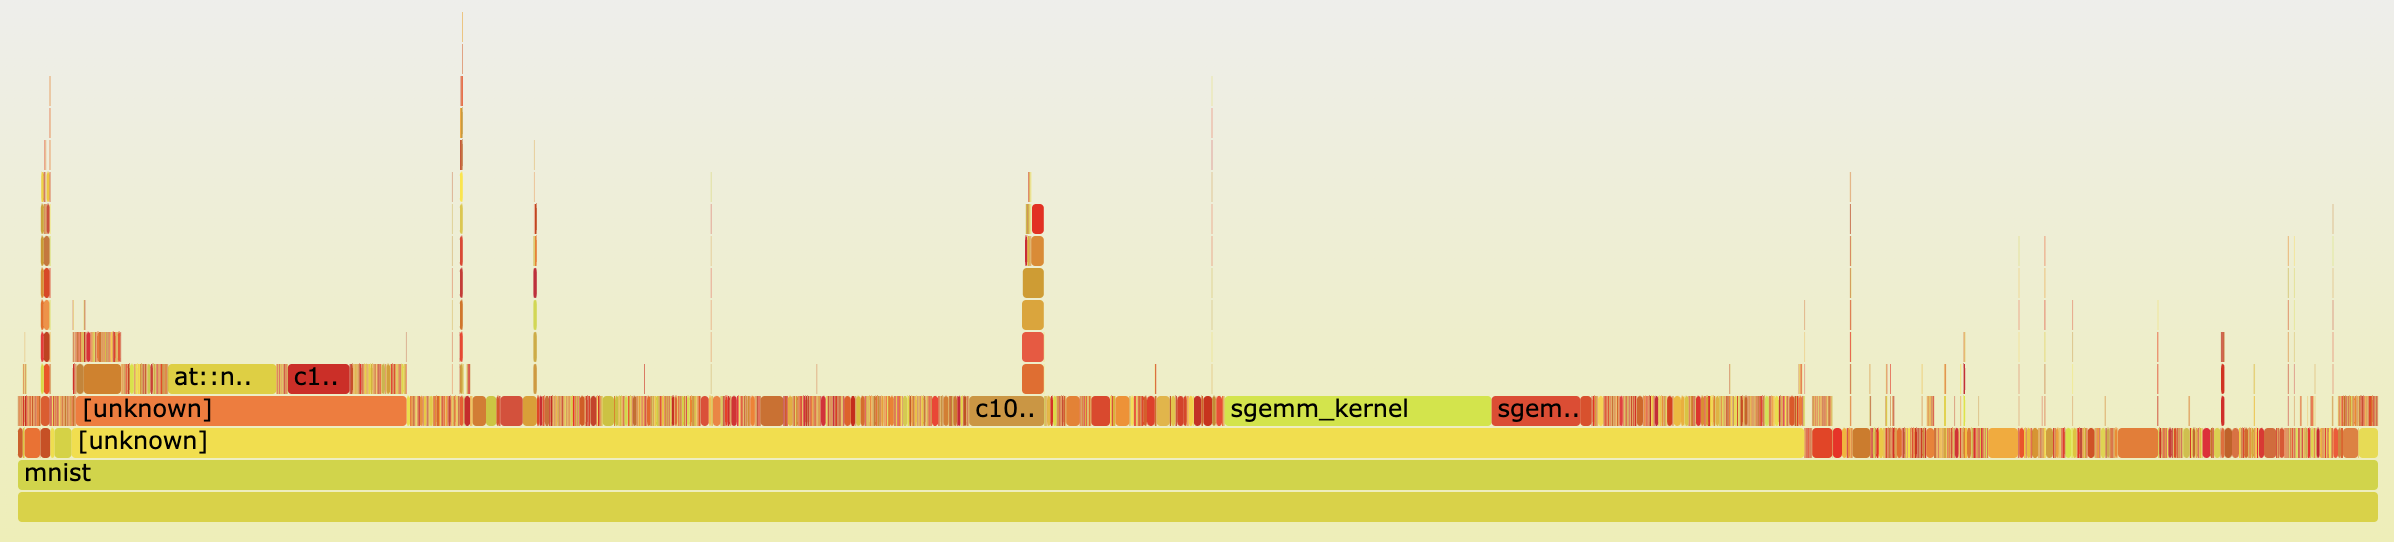
\includegraphics[scale=0.34]{cpp-libtorch-fg.png}
	\caption{cpp-libtorch}
\end{figure}

\begin{figure}[H]
	\centering
	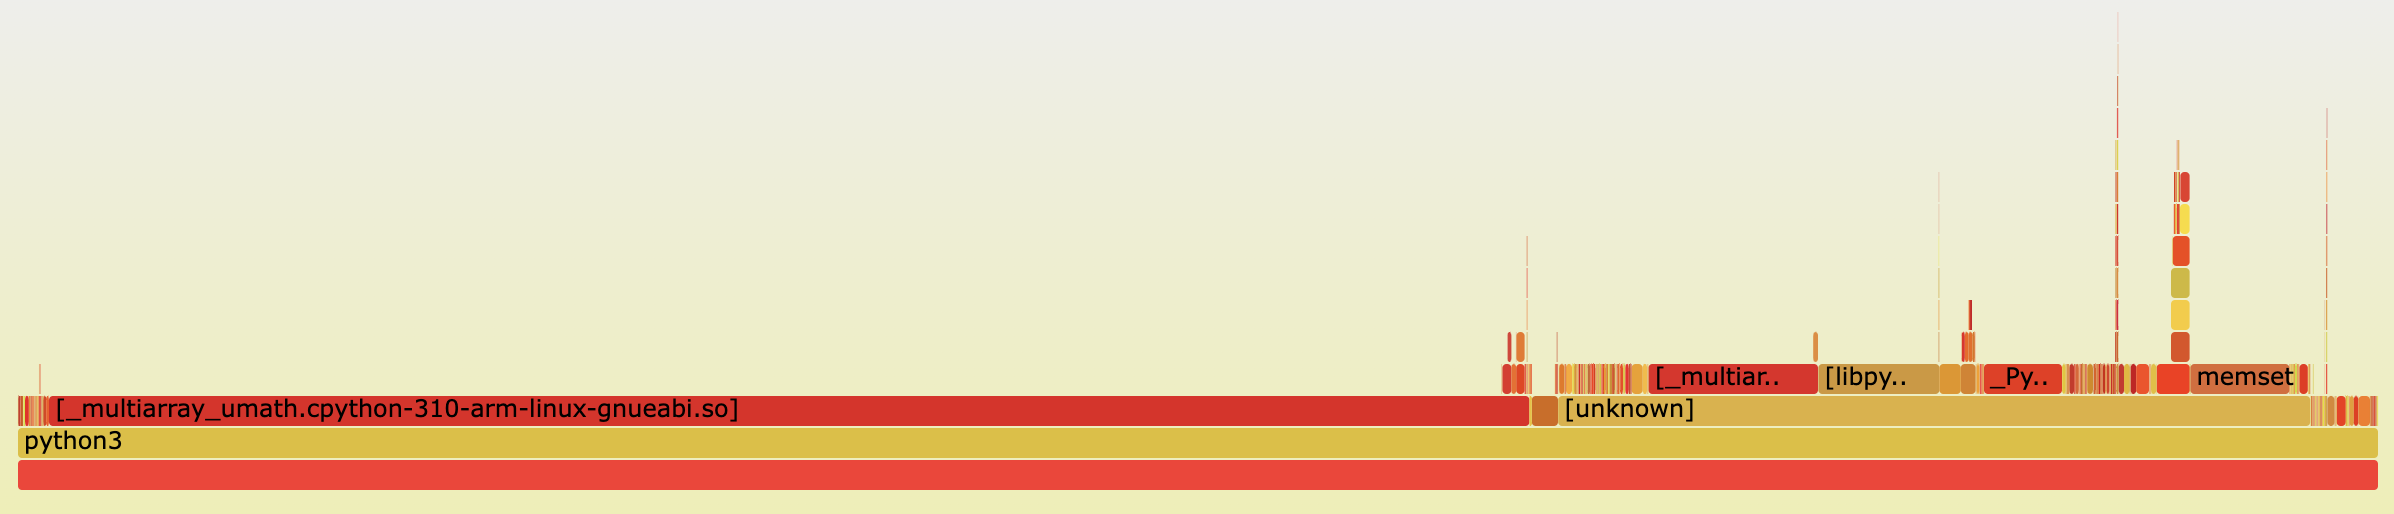
\includegraphics[scale=0.34]{python-numpy-fg.png}
	\caption{python-numpy}
\end{figure}

\subsection*{Memory Profile through Heaptrack} \label{hdrnn-memory-profile}

Heaptrack measurement for C based implementation of HDR-NN running for 4 epochs under different sizes are presented below

\begin{figure}[ht]
	\centering
	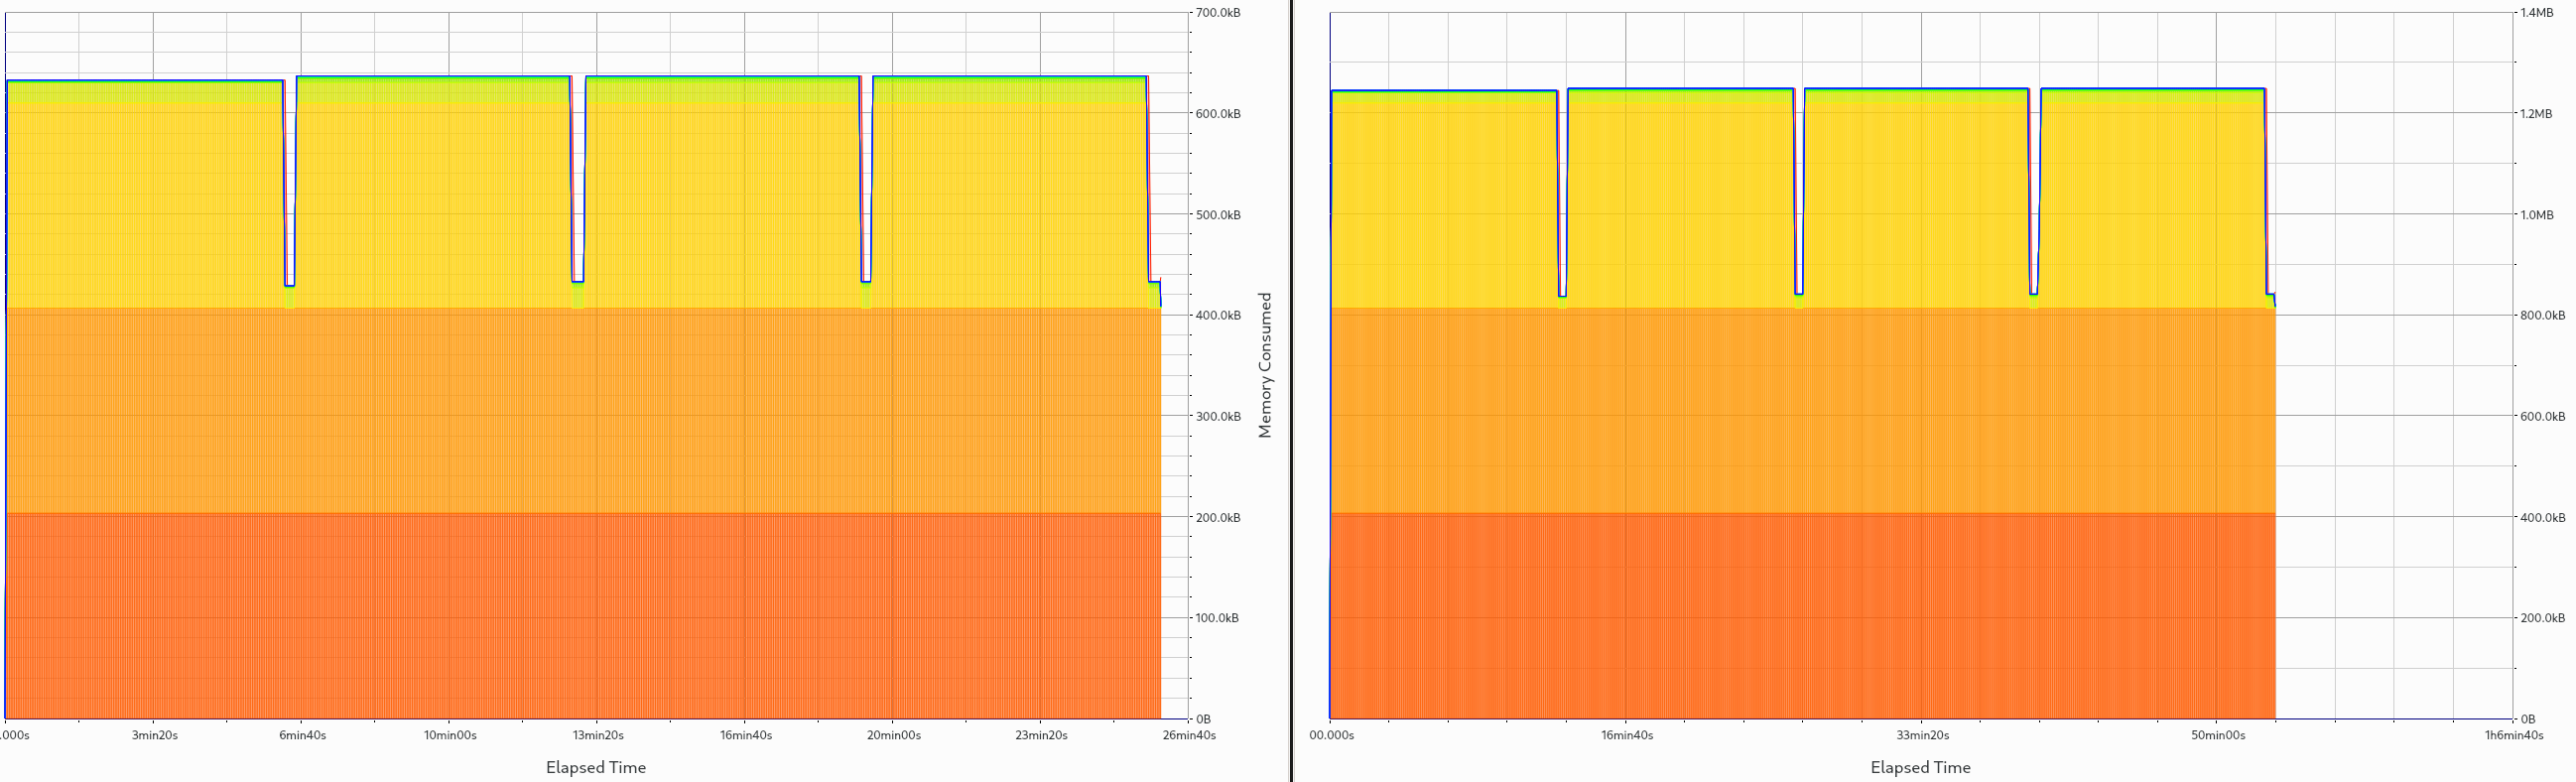
\includegraphics[scale=0.15]{heaptrack-compare.png}
	\caption{c-math.h with 2 different shapes}
\end{figure}

The memory allocations of different size as tracked by Heaptrack for a single epoch execution run of the C based implementation is given below

\begin{figure}[ht]
	\centering
	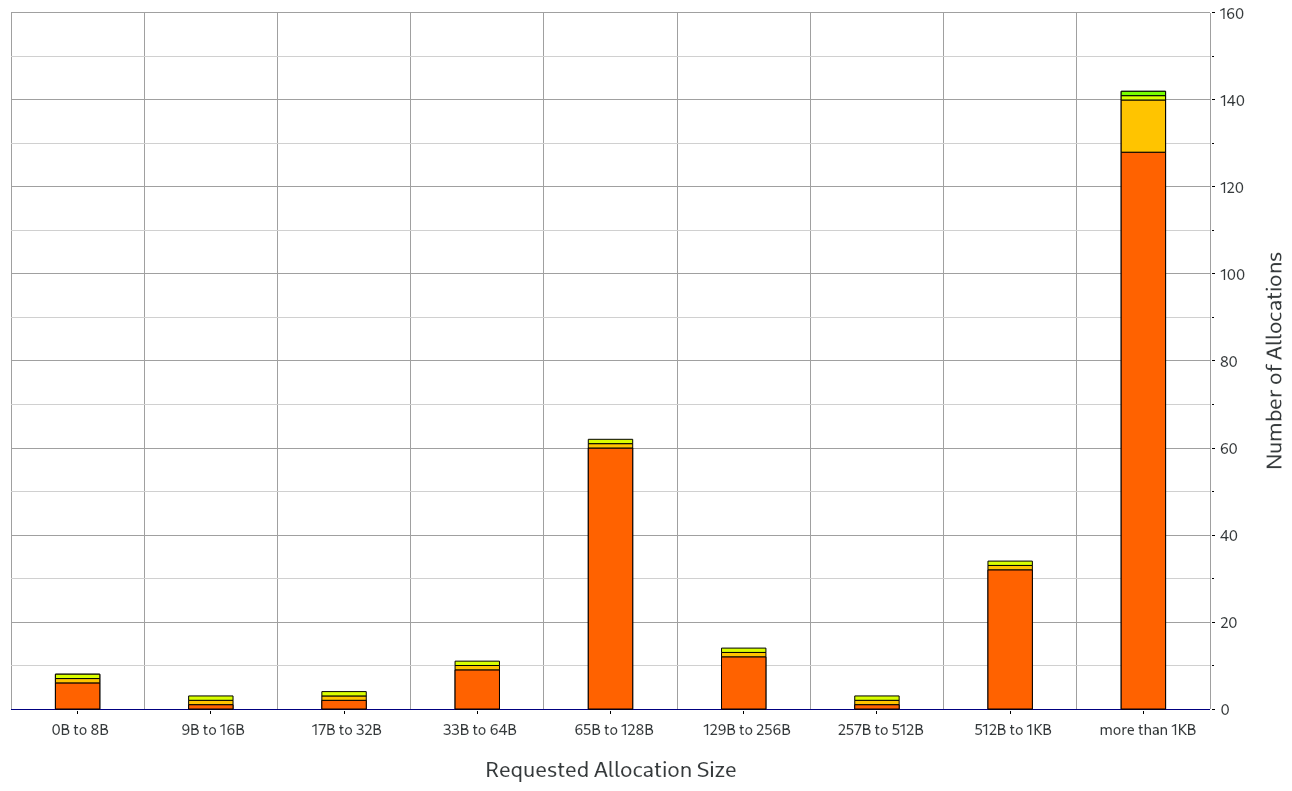
\includegraphics[scale=0.32]{c-math.h-allocations.png}
	\caption{c-math.h allocations}
\end{figure}
